\section{Load balancers in Kubernetes cluster}\label{Load balancers in Kubernetes cluster}

\subsection{Conventional Architecture Problems}

\begin{figure}
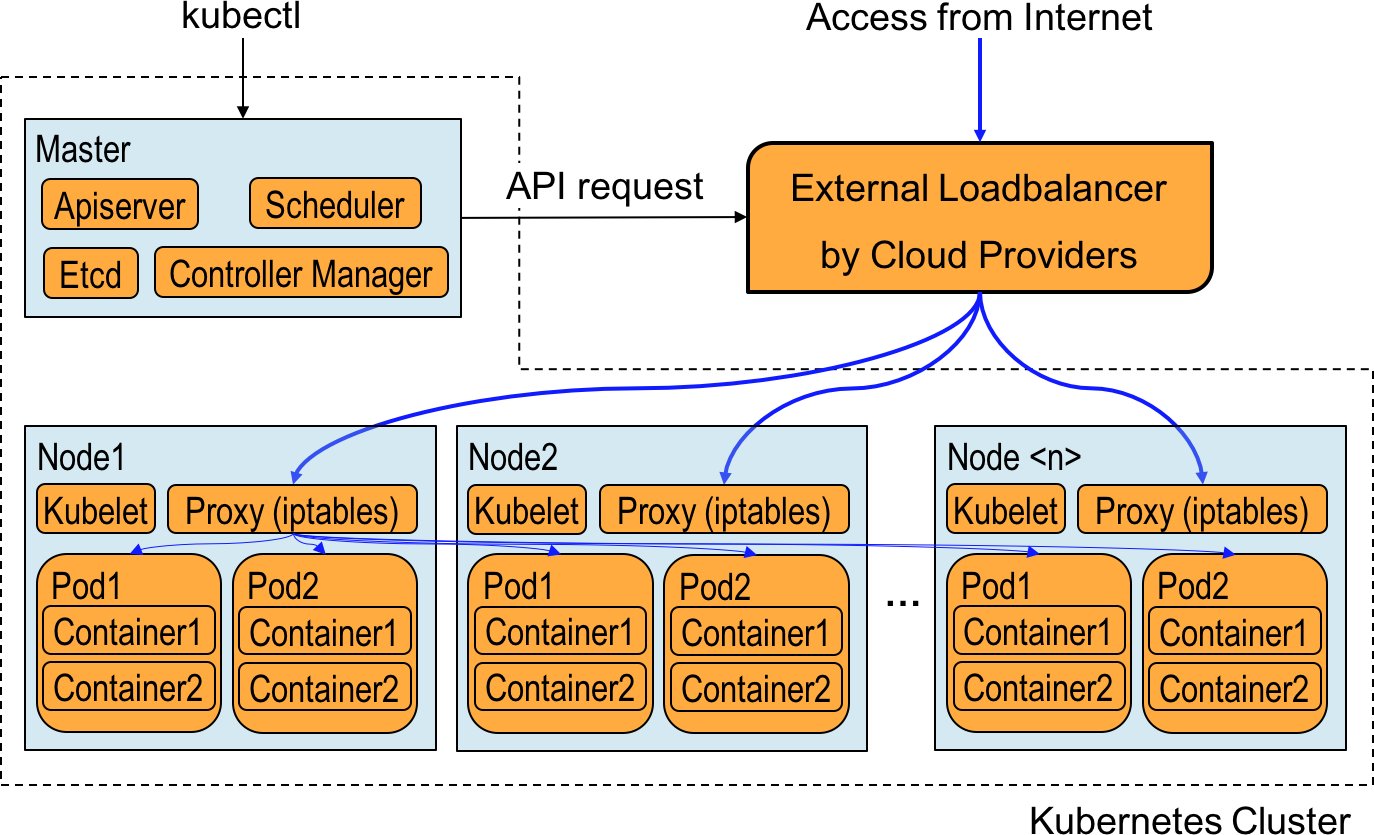
\includegraphics[width=\columnwidth]{Figs/K8sConventional}
\caption{Conventional architecture of a Kubernetes cluster.}
\label{fig:K8sConventional}
\end{figure}

Problems commonly occur when the Kubernetes container management system is used outside of recommended cloud providers(such as GCP or AWS).
Figure~\ref{fig:K8sConventional} shows an exemplified Kubernetes cluster.
A Kubernetes cluster typically consists of a master and nodes. They can be physical servers or VMs.
On the master, daemons that control the Kubernetes cluster are typically deployed. 
These daemons include, apiserver, scheduler, controller-manager and etcd. 
On the nodes, the kubelet daemon will run {\it pods}, depending the PodSpec information obtained from the apiserver on the master.
A {\em pod} is a group of containers that share same net name space and cgroups, 
and is the basic execution unit in a Kubernetes cluster.

When a service is created, the master will schedule where to run {\em pods} and kubelets on the nodes will launch them accordingly.
At the same time, the masters will send out requests to cloud provider API endpoints, asking them to set up external load balancers.
The proxy daemon on the nodes will also setup iptables DNAT\cite{MartinA.Brown2017} rules. 
The Internet traffic will then be evenly distributed by the external load balancer to nodes, 
after which it will be distributed again by the DNAT rules on the nodes to the designated {\em pods}. 
The returning packets will follow the exact same route as the incoming ones.

This architecture has the followings problems: 
1) Having external load balancers whose APIs are supported by the Kubernetes daemons is a prerequisite. 
There are numerous load balancers which is not supported by the Kubernetes.
These include the bare metal load balancers for on-premise data centers.  
In such cases, a user could manually setup the routing table on the gateway so that the traffic would be routed to one of the nodes.
Then the traffic would be distributed by the DNAT rules on the node to the designated {\em pods}.
However, this approach would require complicated network configuration and significantly degrade the portability of container clusters.
2) Distributing the traffic twice, first on the external load balancers and second on each node, 
complicates the administration of packet routing. 
Imagine a situation in which the DNAT table on one of the nodes malfunctions.
In such a case, only occasional timeouts would be observed, which would make it very difficult to find out which node was malfunctioning.   

In short, 1) Kubernetes can be used only in limited environments where the external load balancers are supported, 
and 2) the routes incoming traffic follow are very complex.

In order to address these problems, we propose a containerized software load balancer 
that is deployable in any environment even if there are no external load balancers.
